\chapter{Methodology}~\label{chapter-methodology}
\epigraph{Is there method in the madness?}{Anon (1964--on)}
\buzzwords{Empirical Studies, Theoretical Framework, Conceptual Framework, make assumptions explicit, methodological analysis using prior publications to identify a vocabulary - SE in practice, qualitative analysis,  the 1-2-3 of research design (question - evidence - method) ...}

\begin{wrapfigure}{R}{0.7\textwidth}
  \vspace{-0.75\intextsep}
  \begin{center}
    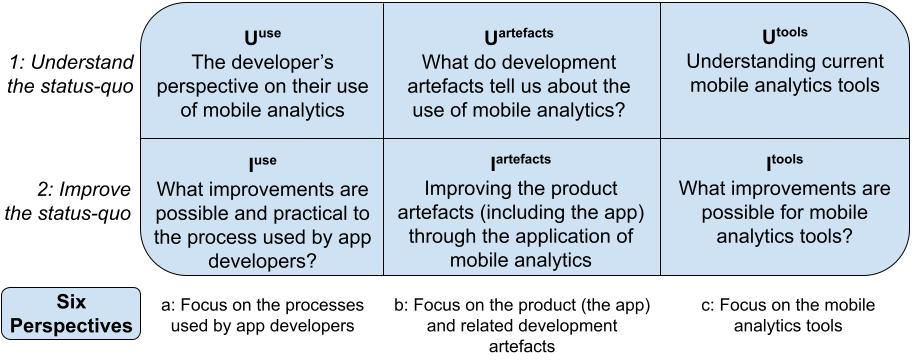
\includegraphics[width=0.66\textwidth]{images/my/six-perspectives-2x3-matrix-12-nov-2021.jpeg}
  \end{center}
    \caption{Methodology six perspectives (repeated)}
    \label{fig:six-perspectives-in-the-methodology}
\end{wrapfigure}

%In the Introduction (page~\pageref{rq-leads-to-six-perspectives}) six perspectives were introduced to support the main research question; these are repeated here in Figure~\ref{fig:six-perspectives-in-the-methodology} for ease of reference. These six perspectives consider three parallel topics: the processes, the products, and the mobile analytics tools in terms of the current practices - their use - and the scope to improve them.
%
%This research applies the 1-2-3 of research design (Question - Evidence - Method) which follow in the next three sections: 

\section{Evidence requirements}
The research needs to provide evidence to answer the main research question: \emph{How can applying analytics improve software development and software testing for mobile apps in practice?} (from Section \ref{overall-research-question}, page \pageref{overall-research-question}). The literature review has situated this question in existing research~\footnote{\textbf{MUST-DO - actually do this!}}.  

Answering this research question requires rich, contextualised evidence of how developers use mobile analytics in practice.  Hence, the research needs to be situated in real-world industry practice and experience, drawing on real-world apps and projects for which analytics have relevance, \textit{i.e.}, that are part of an app-store ecosystem that collects analytics, and that are used by real-world users. The evidence needs to come from the developers, from their app microcosms, and from real-world mobile analytics.

The methodology needs to include techniques that can address the six perspectives introduced in the Introduction (page 9) and repeated here in Figure~\ref{fig:six-perspectives-in-the-methodology} for ease of reference.  Hence, the methodology must 
focus on practical aspects of app development, the use of mobile analytics tools by these app development teams, the quality of these tools, and the value and impact from the perspective of these teams.  Figure~\ref{fig:six-perspectives-in-the-methodology} highlights the needs to both understand the status-quo and to identify potential improvements, with respect to developer practices and thinking, apps and all the associated development artefacts (\textit{e.g.}, source code, issue tracking, tests, and operational configurations) that provide evidence of use, and the analytics tools themselves.

% \newthought{The research needs to be situated in the real-world}
%As the real-world apps live in an app-store ecosystem, and as the main app stores collect app analytics, the research needs to be situated in apps that are available in an app store. And as the analytics are derived from usage the apps need to be used, ideally by real-world users of those apps. 

A comprehensive statistically representative sample of mobile apps was beyond the scope of a PhD, instead `purposeful sampling'.~\citep[pp180-182]{flick2018_an_introduction_to_qualitative_research_sixth_ed}, and more recently in ~\citep[p.114]{zieris2020_phd_qualitative_analysis_of_knowledge_transfer_in_pair_programming}\footnote{\emph{``Unlike for quantitative methods, statistical generalization from a sample to the population is not a goal. Instead, qualitative studies look for information-rich cases that allow to deepen the researcher’s understanding. Early in the process, each case is treated as unique and studied in great detail; cross-case analyses follow later and are based on the well-understood individual cases."}}. 
%
Flick presents six strategies of purposive sampling, in p.181. Of necessity the strategy used in this research is one described by Flick as convenience, however a more appropriate term for the strategy is opportunistic, since few of the case studies were convenient. As Flick notes wryly, on p.182, `the problem of access may be one of the crucial barriers' which particularly applies when seeking access to sensitive data and information about software failures for commercial mobile apps.

Nonetheless in the research I strove to use a variety of projects and apps. The variety is intended to help to uncover emergent features, capabilities, and behaviours; it also helps establish a range of examples of improvements and concerns. 

Further, no two analytics tools are identical; they offer a variety of features and capabilities, and have distinct behaviours.  Furthermore there are tools that work at the platform level and others that work at the app level; researching tools that work at both levels helps determine and distinguish their characteristics and compare their behaviours. Therefore there is value in researching more than one mobile analytics tool.

\section{Data sources}
The nature of research in a sometimes messy real-world environment means access is opportunistic and often occasional. The evidence will be incomplete, yet rich, complex, and multi-faceted. For this research the data sources include:

\begin{itemize}
    \itemsep0em
    \item Development artefacts: app binaries, app source code, tests, work schedules, documentation, bug tracking systems, \textit{etc.}, these were collected during the various case studies and complemented by public sources for additional mobile apps.
    \item `Grey material': online materials on mobile analytics tools, articles including on medium.com and various blogs. Some were found in response to findings during particular case studies, others were found during additional background research.
    \item Pre-study interviews with developers: used for setting up the study, understanding the development context, these were collected as part of the case studies.
    \item mid-study communications with developers: usually email correspondence for clarification, to obtain updates, or comment on observations, these were collected as part of the case studies.
    \item various discussion forums: used by mobile app developers and other online contextual information, online issue tracking and related code for opensource projects beyond those studied in the empirical studies in this research. Some were stimulated as part of the case studies, others were found during additional background research.
    \item field notes: some handwritten, others recorded as text on computers, these were collected as part of the case studies and during background research.
    \item analytics tools: particularly analytics artefacts which include various outputs including screen captures, screen-scraping and parsing, results from calling APIs, and automated emails generated by analytics tools. Product documentation, online help materials, examples, and so on were also used as data sources. These were collected on an ongoing basis during case studies and during additional background research.
\end{itemize}

The evidence is mainly based in real-world cases. For all of these cases, collection of naturally-occurring data (e.g., development artefacts, grey material) was augmented by elicitation of additional data (e.g., interviews and communications with developers) to provide clarification, breadth and insight.  Different research methods made use of these data sources, as appropriate.

\section{Methodology}
Broadly, this research starts from what Ball and Ormerod described as `cognitive ethnography'~\citep{ball2000_putting_ethnography_to_work_cognitive_ethnography}, that is, observation-based enquiry conducted \textit{in situ} to investigate ``...the interplay between people-laden contexts and expert cognition'' (p. 149). Ball and Ormerod characterise cognitive ethnography in terms of observational specificity, verifiability and purposiveness: 

\textit{``Our own conception of cognitive ethnography is characterized by three key features. First, it relies on small-scale data collection based around representative time slices of situated activity. As such, it demonstrates observational specificity, as opposed to the intensity of a prototypical ethnography. Second, it is purposive, in that its mode of questioning focuses on issues that are informed by some intention to intervene with, or somehow affect, existing work practices ... Third, it places a strong emphasis on verifiability, in terms of validating observations across observers, data sets and methodologies.''} (p. 152)

Consistent with this orientation, this research sought to derive a situated understanding of analytics (in terms of the six perspectives in Figure~\ref{fig:six-perspectives-in-the-methodology}). The insights that emerged from the more ethnographically-inspired analysis of naturally-occurring data were then investigated further and tested using other approaches, namely across-case comparison, hypothesis testing (systematic manipulation in local experiments) and action research (evaluation through interventions in specific cases) -- consistent with Ball and Ormerod's emphasis on verifiability.  

\begin{figure}
    \centering
    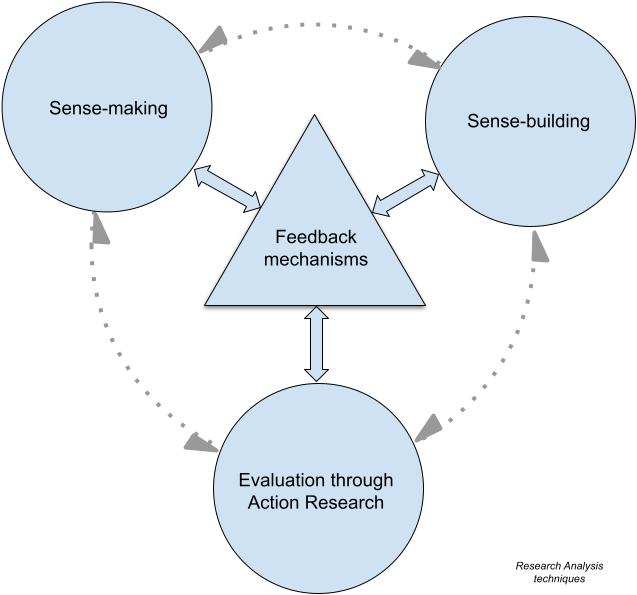
\includegraphics[width=10cm]{images/my/analysis-techniques-in-PhD-08-Nov-2021.jpeg}
    \caption{Categories of research methods}
    \label{fig:categories-of-research-methods}
\end{figure}


 Figure~\ref{fig:categories-of-research-methods} provides a visual overview of the four categories of research methods used to serve this `cognitive ethnography' approach; they include 1) sense-making, 2) sense-building, and 3) evaluation through action research. These were complemented by the fourth category 4) feedback mechanisms to help support and verify the analyses. 
%Categories of research methods (sense-making, sense-building, feedback mechanisms, and evaluation through action research). Each has a distinct purpose which will be discussed in the rest of this section. 

Note: Figure~\ref{fig:categories-of-research-methods} is an over-simplification with clear boundaries between the categories in order to convey the alignment of methods to purposes and the categories are not discrete.  Some methods include several data sources, and some data sources are analysed using several methods. In practice, individual research methods provided multi-faceted contributions; for instance local app experiments contributed to both sense-building and sense-making. 

\medskip

%\subsection{Overview of the research methods}
%Various methods were chosen to address the research needs by engaging with data collected from actual practice, as summarised in Table ~\ref{tab:mapping-analysis-to-six-perspectives}, which groups the methods under their main category, illustrated in Figure~\ref{fig:categories-of-research-methods}, and maps them to the six perspectives. 

Table ~\ref{tab:mapping-analysis-to-six-perspectives} identifies the various research methods, groups them in terms of their roles in the research (as illustrated in Figure~\ref{fig:categories-of-research-methods}), and maps them to the six perspectives.  Each of these research methods includes data collection \textit{and} analysis unless otherwise stated.


\begin{table}
    \small
    \setlength{\tabcolsep}{4pt} %% default is 6pt
    \setlength{\arrayrulewidth}{0.1mm}
    \centering
    \begin{tabular}{l|ccc|ccc}
      & \multicolumn{3}{c|}{\bfseries \small Understand} & \multicolumn{3}{c}{\bfseries \small Improve} \\
      \toprule
         % &\textsubscript{u}Use &\textsubscript{u}Artefacts &\textsubscript{u}Tools &\textsubscript{i}Use &\textsubscript{i}Artefacts &\textsubscript{i}Tools \\
         \multicolumn{1}{r|}{Six perspectives} &\uuse &\uartefacts &\utools &\iuse &\iartefacts &\itools \\ % Thanks to https://tex.stackexchange.com/a/33488/88466
         
        \hline 
        \textbf{Sense-making} & & & & & & \\
        (comprehension and exploration) & & & & & & \\
        Beacon finding and    &Y &y &Y &y &y &y \\
        Drill Down            &y &y &Y &Y &y &y \\
        %\tabucline[1pt on 3pt]  \\ % See https://tex.stackexchange.com/a/109301/88466 however here it is terminated prematurely and a bit heavy 
        % Or try https://tex.stackexchange.com/a/229334/88466 or https://tex.stackexchange.com/a/613907/88466 if I've not collapsed these two previous rows soon.
        % Or use a newer latex package, see https://tex.stackexchange.com/a/611494/88466 

        \hline
        \textbf{Sense-building} & & & & & & \\      
        %(Integration and differentiation)    & & & & & & \\        
        (micro-experiments and macro-discoveries) & & & & & & \\
        Local App Experiments   &y &Y &Y &  &Y &Y \\
        Across Case Comparisons &Y &y &Y &Y &y &y \\        
        
        \hline
        \textbf{Feedback mechanisms} & & & & & & \\
        (triangulation and validation) & & & & & & \\
        Ask The App Devs      &Y &y &y &y &y &y \\
        Ask The Tool Devs     &  &  &Y &y &y &y \\
        Grey Literature Analysis       &y &y &Y &y &y &  \\
        Code Analysis         &y &Y &  &y &y &  \\
                
        \hline
        \textbf{Evaluation through action research} & & & & & & \\
        (embedded intervention) &y &Y &y &Y &Y &y \\
        Observation             &Y &Y &Y &Y &Y &y \\
        Field Experiment        &y &  &  &Y &Y &  \\
        Hackathon               &y &y &  &Y &Y &  \\
        
        \bottomrule
    \end{tabular}
    \caption{Mapping research methods rows to the 6 perspectives columns}
    \label{tab:mapping-analysis-to-six-perspectives}
\end{table}


`\textbf{Sensemaking}' methods were concerned with understanding current practice (as reflected in artefacts, tools, and developers' practices and perspectives -- i.e., perspectives \uartefacts, \utools, and \uuse) and identifying potential improvements in tools and in how analytics are used in app development and maintenance (i.e., perspectives \itools and \iartefacts). The research methods include beacon-finding (see page~\pageref{section-beacon-finding-method}) and drill-down (see page~\nameref{drill-down-research-method}).


`\textbf{Sensebuilding}' methods built on insights found through sense-making. The research methods include local app experiments (see page~\pageref{local-app-experiments-research-method}) and across case comparisons (see page~\pageref{across-case-comparisons-research-method}).

Micro-experiments (i.e., local app experiments) are used to investigate detail and give insight into the relationships between tools, quality of analytics, and potential impact of analytics use on apps (i.e., perspectives \uartefacts, \utools, \iartefacts, \itools).

Across-case comparisons identify macro-discoveries -- that is, they identify characteristics and patterns that were not evident in individual case studies, potential improvements to practice (i.e., perspectives \uuse and \iuse), as well as the influence of the quality of tools in practice (\itools). They can also corroborate and/or challenge findings found in individual cases.


`\textbf{Feedback mechanisms}' were used to support and verify the other analyses, by comparing observations to other evidence, or by asking developers for clarifications or reflections. Feedback mechanisms are used throughout the research and mainly used for perspectives that sought to understand (\uuse, \uartefacts, and \utools), nonetheless they were also frequently used when considering improvements (\iuse, \iartefacts, and \itools). 

`\textbf{Evaluation through action research}' methods were largely concerned with evaluation of the effect of improvements in the use of analytics, in terms of adoption into use and app performance (i.e., perspectives \iuse and \iartefacts). It includes three research methods: 1) observation, 2) field experiment, and 3) hackathon. These are explained in page \pageref{section-evaluation-through-action-research-method} onwards. 

The research is iterative, moving through sensemaking, sensebuilding and feedback mechanisms repeatedly as new cases are studied or new insights emerge.  The methods and the data sources often also inform several of the six perspectives.  The research methods are introduced in more detail in the sections that follow.

\subsection{Sensemaking}
% c.f. https://en.wikipedia.org/wiki/Sensemaking_(information_science)
%1) Identifying patterns (inductive analysis) c.f. grounded theory. 2) 

`Sensemaking' includes 1) beacon finding and 2) drill down. These were used for \textit{inductive analysis} of artefacts, broadly consistent with grounded theory [amplify this...].  These methods were amplified through the feedback mechanisms, covered shortly. 
%In addition a third method, local app experiments, was used to create conditions for additional sensemaking.

%Sensemaking has been applied to various aspects of computing and software development, for example: in program comprehension, in understanding end-users' understanding of spreadsheets~\citep{grigoreanu2012_end_user_debugging_strategies_a_sensemaking_perspective}. COULD-DO discuss the work of~\citep{naumer2008_sense_making}. Our use of sensemaking is inspired by sensemaking in research into these areas. 

%The following methods primarily helped with sense-making: analysing and ``making sense" of mobile analytics tools, development artefacts, and the developers' perspectives on their use of mobile analytics. 

\subsubsection{Beacon-finding}~\label{section-beacon-finding-method} %concept, adaption to suit this research, examples.

The notion of \textbf{`beacons'} was borrowed from research on program comprehension; for instance by Wiedenbeck, who helped establish beacons in software development: ~\emph{``In programming, beacons are lines of code which serve as typical indicators of a particular structure or operation"}~\citep[p.679]{WIEDENBECK1986_beacons_in_computer_program_comprehension}. The work was extended and updated to explicitly consider the effects of beacons in comprehension of source code, for instance in~\citealt{crosby2002_roles_beacons_play_in_comprehension_etc}.

The notion of beacons was generalised for this research to include indicators in the analytics of something of interest, or something that required attention.  And so 'beacon finding' was an inductive process by which significant indicators in the analytics data were used to identify areas of the code base that required further investigation.  Mobile analytics may include source code that calls APIs in the application's source code, however the bulk of the contents that need to be comprehended comes as outputs from the mobile analytics tools, therefore the beacons will differ accordingly. In this research the beacons include: the shape of graphs in mobile analytics report, failure clusters, a method call in stack traces, and so on.

%\marian{Now specify how you spotted beacons... I looked for things on this basis, how I kept track of things, what selection criteria were used and why?}

Beacons emerge in various ways. For instance in reports they include: anomalies within a report, mismatches and inconsistencies between two sibling reports or between a master report and the linked detailed report, in the shape of the curve of a graph, in the distribution and groupings of aggregate data, and so on. Similarly, alerts as determined by a mobile analytics service may be considered potential beacons being `promoted' by the mobile analytics reports. 

The most common method of recording potential beacons was using web browser screenshots and/or other mechanisms that preserved information electronically. Some were annotated as part of the beacon-finding and drill-down analysis. Additional notes were written both electronically and/or in physical notebooks. 

Selection criteria included: top ranking results, atypical rates of change, adverse changes to reliability, novel failures particularly for the most recent release, etc. A consistent and overriding criterion was to seek beacons that indicated flaws and failures that could materially and adversely affect the user experience of the app for one or more users of the app.

\julian{c.f. Cognition in the wild, as a parallel example of rich and emergent findings from the real world that would be very hard to specify or determine the factors that applied at the time the ship was being brought under control~\citep{hutchins1995_cognition_in_the_wild}.}

%\textbf{Beacon finding} seeks potentially relevant indicators, typically within bounded domain such as software code. Beacons help to convey meaning and are used for comprehension, for instance by programmers who wish to understand source code~\citep[page i]{crosby2002_roles_beacons_play_in_comprehension_etc}. The concept of beacons in source code has been studied by various authors for several decades; for instance by Wiedenbeck, who helped establish beacons in software development: ~\emph{``In programming, beacons are lines of code which serve as typical indicators of a particular structure or operation"}~\citep[p.679]{WIEDENBECK1986_beacons_in_computer_program_comprehension}. The work was extended and updated to explicitly consider the effects of beacons in comprehension of source code, for instance in~\citealt{crosby2002_roles_beacons_play_in_comprehension_etc}.
 


% I'm not sure where to discuss beacons in conversations: for instance in a developer's description of their use of mobile analytics to assess the quality of the app - they exist to me - TBD.


\subsubsection{Drill-down}~\label{drill-down-research-method}
Beacons stimulate interest, the interest needs to be satisfied one way or another by investigating the beacons and their underlying information sources. 
Are the identified beacons genuinely significant, what do they signify or relate to in the app and its usage, etc.  Drill-down start with the original data sources, but may draw in others to clarify relationships, responses by the developers, etc.

 

Here are 2 examples: 1) investigating a large spike in the overall crash rate to determine the constituent causes (\textbf{TODO} add link to an actual example in a case study); 2) understanding a Java WebView Exception (\textbf{Again TODO} provide a link to the example in my thesis). 


\subsubsection{Sensemaking and decision-taking by developers}
Before we move on to the category of sense-building one of the insights from the research is the use of similar sense-making by developers when they use mobile analytics as inputs to their development work and as feedback for [their] previous development work.

\begin{figure}
    \centering
    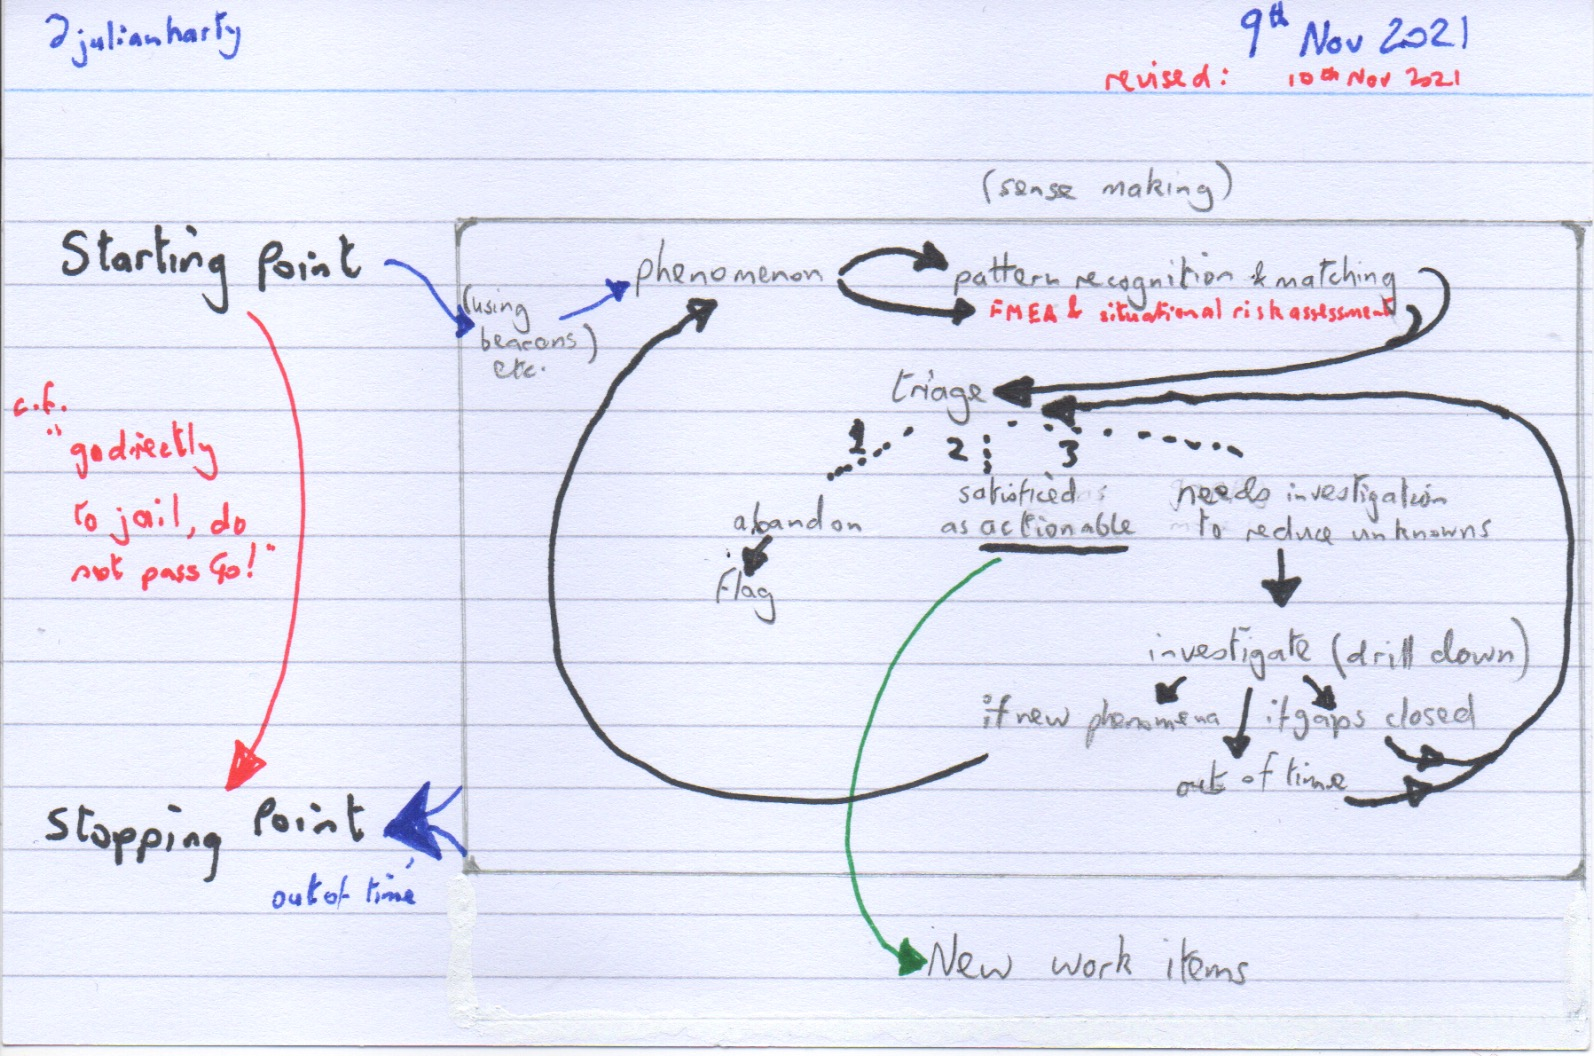
\includegraphics[width=15cm]{images/rough-sketches/practical-sense-making-process-10-nov-2021.jpeg}
    \caption{Sense-making process when development teams apply mobile analytics}
    \label{fig:practical-sense-making-process-when-dev-teams-apply-mobile-analytics}
\end{figure}


Figure~\ref{fig:practical-sense-making-process-when-dev-teams-apply-mobile-analytics} illustrates the sense-making and triage process used by development teams which shares various similarities with sense-making from a research perspective. These similarities mean the researcher and the practitioner may also share similar practices in terms of their analysis of phenomena found in mobile analytics tools. The triage and drill-down may be repeated several times where there is sufficient potential value in performing further investigation. 

The impact of reported failures is combined with situational-risk-assessment as a part of the decision-making process performed by developers during triage; for instance to consider whether this reported issue is worth addressing in the current development cycle, (\textit{e.g.} in the current Sprint for teams who use Sprints for work planning. Developers have to consider multiple criteria including personal, project, and product implications of making code and/or operational changes.

As an untested hypothesis, as part of their decision making when triaging an issue: developers may apply an informal form of failure mode and effect analysis (FMEA) based on multiple-criteria decision making (MCDM) using similar criteria to the work described in \citealt{lo2018_novel_multi_criteria_decision_making_based_FMEA_model_for_risk_assessment}, \textit{i.e.}, severity, occurrence, detection (of a cause they can fix), and expected cost. An area of future research could be in the habits of decision making during triage and in ways to improve the decision making and the outcomes of those decisions.

\subsection{Sense-building}
%\akb{need an introductory paragraph here that explains how sense-building is different from sense-making, and an overview of the activities included in this part of the analysis}

Sense-building moves beyond sense-making. Sense-making aims to understand \textit{what is} while sense-building involves direct action and more active research, for instance: to devise and run experiments to learn more about the behaviours of mobile analytics, and to seek patterns and generalisations across tools, case studies, and so on. Two methods were used primarily in sense-building: local app experiments and across-case comparisons. 

\subsubsection{Local-app experiments}~\label{local-app-experiments-research-method} 
\textbf{Local app experiments} were used to \textit{test the understanding} of the relationships between the usage and the analytics through manipulations of apps and observation of the effects -- hence, the local app experiments were used to test some of the patterns identified in the inductive analysis.

\textit{Micro-experiments} (i.e., local app experiments) were created by developing small mobile apps intended to exercise particular aspects of mobile analytics~\footnote{Similar to the `invent the future' adage, for example: \url{https://quoteinvestigator.com/2012/09/27/invent-the-future/}}). The inputs to an app were directed in order to determine the outputs from mobile analytics. These helped to answer questions and gaps observed as part of sensemaking.  The local app experiments gave insight into the relationships between tools, quality of analytics, and potential impact of analytics use on apps (i.e., perspectives \uartefacts, \utools, \iartefacts, \itools). 

Local-app experiments used small mobile apps, not intended for production use, that were developed in order to investigate the relationships between the inputs (such as usage) and the analytics outputs (such as reports) through deliberate manipulation of the inputs and observation of the consequences.  
 The local-app experiments allow for tighter control on the usage, \textit{i.e.} the inputs, in comparison to the unfettered use of real-world mobile apps. They can help surface behaviours and provide for tighter evaluation in the early, pre-launch/pre-production phases. %I can't say feedback as that'd conflate the other use of feedback here in the methodology.
The local app experiments were used to test some of the patterns identified in the inductive `sensemaking' analysis.

Where practical the source code of these apps is made available under a permissive opensource license to facilitate further research by others and in order to facilitate inspection by and feedback from others.


\akb{Also explain how the results of these experiments connected to other parts of the method? e.g., did they change / add to the sense-making activities?}

\subsubsection{Across-case comparisons}~\label{across-case-comparisons-research-method}
\textit{Across-case comparisons} were concerned largely with understanding current practice and identifying potential improvements to practice (i.e., perspectives \uuse and \iuse), as well as the influence of the quality of tools in practice (\itools).

Similar to using various software testing techniques to find bugs, making comparisons across the case studies can help to identify more of the behaviours of mobile analytics, their use, and their efficacy. Across-case comparisons can increase the probability of seeing fresh characteristics and establish similarities across cases. The comparisons across case studies help establish norms (which can also be used to identify beacons, and anomalies), patterns (and anti-patterns), variety, and ranges. 

While comparisons across cases (\textit{i.e.} across projects and their mobile apps) can help developers they particularly help with/from the research perspective.

\begin{itemize}
    \item \textbf{For developers}: they can compare the reports for their apps with the results others obtain. Doing so may help them identify problems-in-common (shared problems) and fixes-in-common that work for many apps with similar failures. They can also establish norms and the comparisons help provide triangulation and perspective. Some developers also find peer-group comparisons stimulating.
    
    \item \textbf{For researchers}: across case comparisons include `plus one'~\citep[pp 28-29]{aurini2016_how_to_of_qualitative_research} research that can help uncover emergent behaviour, reinforce existing findings, and so on. The across case comparisons also provide additional microcosms where new findings are discovered in the behaviours of apps, the tools, the development practices, and the efficacy of the use of mobile analytics performed by a wider variety of development teams.
\end{itemize}

\begin{figure}
    \centering
    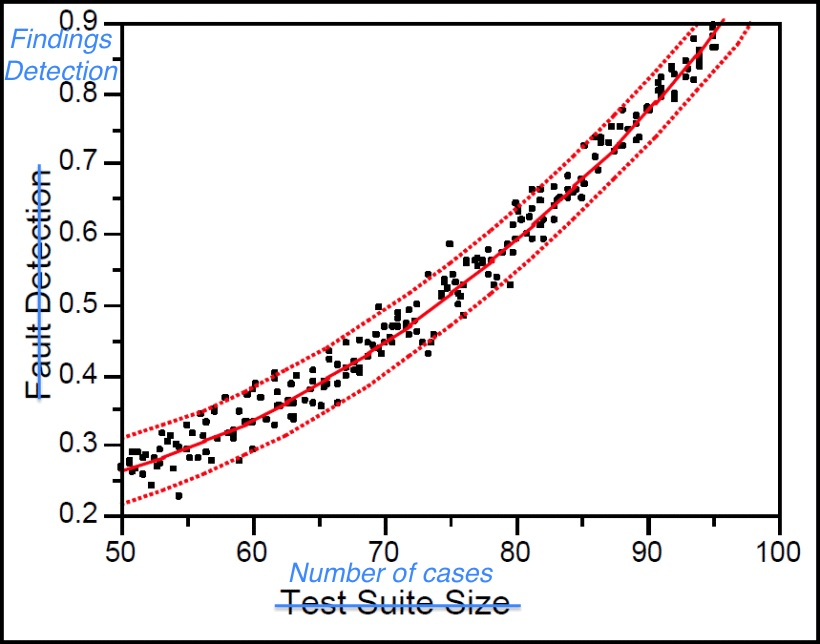
\includegraphics[width=10cm]{images/rough-sketches/across-case-comparisons.jpg}
    \caption{Across case comparisons behaviour detection curve \\Hack of Figure 2 in \citep[p.2]{briand2007_a_critical_analysis_of_empirical_research_in_software_testing}}
    \label{fig:across-case-comparisons-behaviour-detection-curve}
\end{figure}

The data and the system state for individual apps can help to increase the `coverage criteria' for a mobile analytics tool (which may be considered a system or simply a `box' as in black-box, grey-box, or white-box system). We know from related domains that more cases can increase the detection rate. For example, a paper by Briand~\citet{briand2007_a_critical_analysis_of_empirical_research_in_software_testing} discusses concepts including the cost-effectiveness curve. A similar approach of recognising the relationship between the number of cases and the detection of pertinent behaviours is illustrated by Figure~\ref{fig:across-case-comparisons-behaviour-detection-curve}. A key observation is that detection is not static nor a one-off value; behaviours come and go, particularly in mobile analytics tools where reports are often ephemeral. The value of across-case comparisons increases when the sampling increases to record more of the ephemeral behaviours and outputs.

The nature of this PhD research based on a relatively small number of apps and associated case studies means it is premature to attempt to systematically plot the number of cases against the behaviours that were observed. Instead the focus is on monitoring 
new insights vs. resonance, and how often a new case highlights something that I'd missed in previous ones~\footnote{\textit{c.f.} Testing and Noticing~\citep{bolton2009_testing_and_noticing} which discusses noticing from a software testing perspective.}? Does anything generalise beyond a single case? % c.f. OFAT and MFAT in bug investigation. 
% An interesting read from mechanical engineering on OFAT and MFAT https://doi.org/10.1016/j.engfailanal.2019.04.002 

\subsection{Feedback mechanisms}
Four methods were used to obtain feedback, two involved asking humans and the other two interrogated existing materials created (mainly) by humans.

\phantomsection
\label{method-vectored-questions}
%A method termed `\textbf{vectored analysis}' was used with both app developers and and analytics tool developers, \textit{i.e.} during two of the feedback methods: 1) ask the app devs, and 2) ask the tool devs. 
Vectored observations/questioning/analysis was used with the aim of increasing the understanding of their work pertaining to mobile analytics. Vectored questions are purposeful and focused, they are similar to Petre's `targeted observation'~\citep[p.234]{petre2009_insights_from_expert_software_design_practice} and situated in the actual practice of the developers - their real world microcosm. They draw on multiple data sources which allows for comparison/triangulation/colligation and allows for multiple methods to gather and analyse data -- all with a focus on the research questions.

Feedback mechanisms, corroborate and challenge... - calibrate with the developers. c.f. experts are also the users and asked if they recognise and agree with particular findings. 


\subsubsection{Ask the app devs}~\label{section-ask-the-app-devs-research-method}
The developers of the apps are uniquely able to voice their perceptions and thinking on their use, experience, and perceptions of using mobile analytics. They are therefore well placed to provide feedback on their use of mobile analytics and also answer questions about their use of mobile analytics in their development artefacts and their perceptions of the mobile analytics tools.

They are also busy with their challenges related to developing and improving the mobile apps they are responsible for. As Petre notes~\citealt{petre2009_insights_from_expert_software_design_practice} the experts are willing to try/explore many tools however they focus on what can help them, and they may discount many aspects of the mobile analytics tools including some of the characteristics and behaviours of interest from a research perspective. Nonetheless from a research perspective it may be useful to learn more about why they have discounted or rejected various aspects of the tools. 

\subsubsection{Ask The Tool Devs}~\label{section-ask-the-tool-devs-research-method} 
%  &  &  &Y &y &y &y \\
The tool developers understand their mobile analytics tools in depth and many have a unique vantage point to observe how their mobile analytics behaves across a large population of apps. Furthermore they are well placed to design, implement, and release fixes and improvements to their mobile analytics products and services. They understand the rationale of their mobile analytics tools and their user-base. And yet, they do not know everything about how their tools are used or perceived and many are keen to receive feedback and insights accordingly.

The research method entails communicating with knowledgeable, available and interested people who develop (in the broad sense) the relevant mobile analytics tool. The communication may be direct or indirect (for instance via their customer service, via online feedback links, or in the form of contributions to their opensource project). Being able to provide succinct, clear, timely, and relevant communications may increase the chances of engaging in a mutually productive dialogue.

\subsubsection{Grey Literature Analysis}~\label{section-grey-literature-analysis-research-method}   
%   &y &y &Y &y &y &  \\
A great deal of grey literature, and grey data~\citep[pp 219-221]{banks2010_blog_posts_and_tweets_the_next_frontier_for_grey_literature}, is available online, covering mobile analytics and to errors, problems related to source code and libraries used in real-world mobile apps. The main sources of relevant grey data include Stack Exchange websites frequented by mobile app developers (particularly \href{https://stackoverflow.com/}{stackoverflow.com}) and GitHub. 

Both Stack Exchange and GitHub provide comprehensive and useful search capabilities which help find relevant content, for instances examples where other development teams have found, understood, and addressed particular crashes in their Android app that also apply to the app in the case study.

\href{https://stackoverflow.com/}{stackoverflow.com} provides facilities that encourage meta-data to be provided by users of the site \textit{e.g.} tags, votes, accepted answer flag, \textit{etc.} and their search provides facilities to perform searches that use meta-data as well as free text~\citep{stackoverflow2021_search_help}.

The nature of GitHub projects provides some inherent structure which can be utilised when performing searches, for example to search issues and pull requests~\footnote{\href{https://docs.github.com/en/search-github/searching-on-github/searching-issues-and-pull-requests}{Searching issues and pull requests}}. GitHub uses the term `qualifier' in the online documentation~\citep{github2021_searching_code_github_docs}, and the terms `prefix' and `tag' in their online search page \url{https://github.com/search} to describe their mechanisms to filter the search results. 

% Crashlytics search should be mainly matched in Android projects because of the target filename. https://github.com/search?q=crashlytics+filename%3Abuild.gradle&ref=simplesearch 

% If I ever have the time and purpose, continue trying to use https://sourcegraph.com/search in case it's able to perform the searches we did in our joint research. Ditto try again with github's v4 search API.

\subsubsection{Code Analysis}~\label{section-code-analysis-research-method}   
%       &y &Y &  &y &y & \\
Source code provides a snapshot of raw ingredients which is used by the development team's build process in order to generate an app. The source code often includes at least one build `recipe'~\footnote{For most Android apps the main build recipe is in the file \texttt{./app/build.gradle}.} so the build can also be evaluated and hopefully reproduced~\footnote{Aside from sensitive ingredients such as signing keys used to digitally sign each binary when it is created.}. The source code's repository provides augments the source code by recording the historical evolution of the source code.

Code analysis in the context of mobile analytics involves searching for indications of the use of one or more in-app mobile analytics libraries. The steps performed to identify indicators %c.f. beacons as used in this chapter
of the use of a mobile analytics library include:

\begin{enumerate}
    \itemsep 0em
    \item Details in one or more \texttt{gradle} scripts where the analytics is added as a `dependency', the version of the dependency provides useful meta-data on whether the analytics are actively maintained by the developers. % COULD-DO\textit{e.g.} add code snippet e.g. see https://firebase.google.com/docs/analytics/get-started?platform=android#add-sdk
    \item Initialisation of the analytics library in the source code, often this occurs in the Android app's \texttt{Application} class. % Ditto there's an example code snippet at https://firebase.google.com/docs/analytics/get-started?platform=android#add-sdk
    \item \texttt{Import} statements in individual source code files that reference the analytics Java package(s).
    \item Searching for one or more \textit{wrapper} class files. If these exist then extend the search for these custom classes in step 3 and 5.
    \item Search for calls to the original and any wrapper mobile analytics API classes. % e.g. based on examples including https://firebase.google.com/docs/analytics/get-started?platform=android#start_logging_events
\end{enumerate}

After the five steps have been completed the matching lines of source code are then available for analysis. 
%
The analysis can be performed for any snapshot of a codebase \textit{i.e.,} for any commit made to the version control repository. Commands such as \texttt{git blame} provide information of the particular commit where lines of code were last updated and complement analysis of the snapshots.

The application of five steps can be scripted. As an example, in joint research~\citep{harty2021_logging_practices_arxiv} a mix of manual and scripted steps were applied to enable the analysis of the use of Firebase mobile analytics in all the commits made to 57 opensource Android apps.

A useful confirmatory test to help establish the integrity of an app's codebase is to build the app using the build scripts. There may be additional documentation of the build process available \textit{e.g.} in a README file incorporated into the code base.

\subsection{Evaluation through action research}~\label{section-evaluation-through-action-research-method}
The article by ~\citet*{avison1999_action_research} on Action Research explains the utility and importance of Action Research in order to establish the relevance of academic research by trying out theories with practitioners in real situations and in real organisations. They recommend action research \emph{``because this [articular qualitative research method is unique in the way it associates research and practice, so research informs practice and practice informs research synergistically."}~\citep[p.94]{avison1999_action_research}. Action research is particularly relevant for the evaluation where it \emph{``encourages researchers to experiment through intervention and reflect on their intervention and the implication of their theories."}~\citep[p.95]{avison1999_action_research}. 

The case studies include examples where the researcher's mode of engagement was as:
\begin{enumerate}
    \itemsep0em
    \item a consultant and/or an embedded developer: an active participant integrated into the project team,
    \item a coach: of an existing team of developers who applied the concepts,
    \item an interviewer: of various development teams to learn of their practices and results,
    \item an analyst/observer: performing static analysis of opensource code repositories~\footnote{Analysis of proprietary code repositories is also possible, but not practicable for this research owing to confidentiality agreements.}.
\end{enumerate}
%\isabel{I think if you look at this in terms of the methodology, you can weave in some of the things Aurini, Heath, and Howells talk about. So in the first two points the research is "of me" whereas in points 3 and 4 it is not.}
\isabel{From Clough and Nutbrown, in points 1 and 2 the way you can be political and persuasive is different to how you apply political/persuasive as a result of 3 and 4. When you are a coach the point of being in the project is to effect change. The research effects change as a result of how you promulgate the results}

%TODO complete the following thought: Research effecting change when I am an active part of it, i.e. in 1 and 2 above.

\subsubsection{Observation}~\label{section-observation-research-method}
\julian{The following example needs moving to a later chapter once I've sketched out the research equivalent of Figure~\ref{fig:practical-sense-making-process-when-dev-teams-apply-mobile-analytics}.}
Many of the developers were often satisficed with what the mobile analytics tools reported - where they accepted local optima (determined through a combination of observation and asking the app devs), \textit{e.g.} they accepted the `top' crash cluster as the worst one. Therefore, if there are flaws in what is being reported the effects of those flaws may permeate into the results of what the developers \textit{do} and \textit{don't} do. 

\subsubsection{Field experiment}~\label{section-field-experiment-method}
In this research, field experiments use real-world apps and their core code repositories. They were not as rigorous as controlled experiments owing to the nature of the development teams and their priorities. Nonetheless they included a control app and an experiment app where experiments are performed on the experiment app and mobile analytics results compared for both these apps. They are also ecologically valid, ~\citep[p.126]{Ko2015_a_practical_guide_to_controlled_experiments_of_sw_eng_tools_with_human_participants}, as they are situated in real world challenges in real world apps.

The approach described in~\citep{Ko2015_a_practical_guide_to_controlled_experiments_of_sw_eng_tools_with_human_participants}: were not suitable. My research didn't have the opportunity to compare two tools quantitatively, nor was it practical to perform quantitative research experiments as none of the projects were interested in the complexity and demands of the type of controlled experiments illustrated in their research. This form of research may be useful and also viable for large, funded research groups and/or for organisations such as the larger mobile analytics tool providers, particularly Google. That said, Google in particular has access to such a vast range of data about the use of their mobile analytics tools they may not need or want to perform controlled experiments of the form discussed in this research.

% Stuff to read?
%
%


\subsubsection{Hackathon}~\label{section-hackathon-research-method}
The hackathon research method in this research applies the concepts of software development hackathons with the addition of mobile analytics tools as a source of information related to issues in the behaviour of one of more mobile apps supported by participants in the hackathon.

The hackathons were communal+contributive+catalytic, see: \emph{`` communal (towards  community  nurturing), contributive  (issue-oriented),  or  catalytic  (towards  the search  for  innovation)."}~\citep[p.3]{medina2020_what_do_we_know_about_hackathons_etc_a_SLR}~\footnote{Note: The source of these terms appears to be in `A Typology of Hackathon Events' a paper published via \url{https://hackathon-workshop.github.io/}, however the actual PDF is on Google Drive and access is restricted. I have requested a copy via Google Drive and from one of the authors.}.
% The 2nd workshop is no longer online, instead see https://web.archive.org/web/20181203070803/http://hackathon-workshop-2018.com/ 

No rewards were offered to participants beyond being at the respective hackathon and participating. These are termed `Single-Application' hackathons in~\citealt[p.5]{briscoe2014_digital_innovation_the_hackathon_phenomenon}. The participants were current members of the respective development team.

In the context of this research the hackathons included the researcher and a highly experienced leader and contributor in previous hackathons. They prepared much of the hackathons together; and in one case (PocketCode) co-led the hackathon. The app, topic, and focus were both selected as part of the preparations. The work during the hackathon was determined by the participants with guidance and suggestions from the organisers.

% https://hackathon-planning-kit.org/ 


\begin{figure}
    \centering
    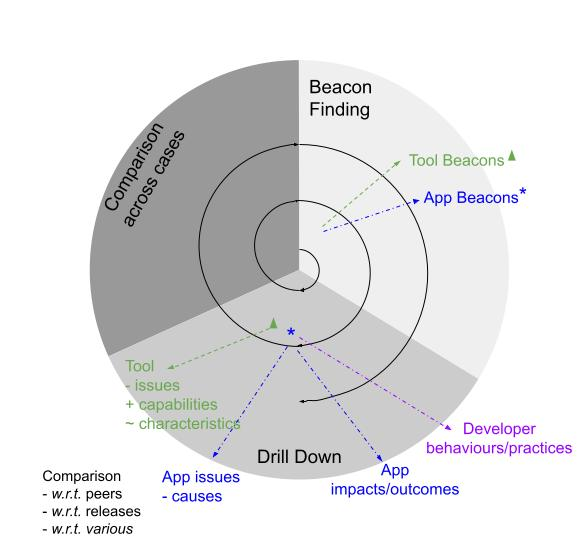
\includegraphics[width=14cm]{images/my/Illustrated-Research-Methodology-using-Mobile-Analytics-as-the-Epicentre-v0-2.jpeg}
    \caption{Illustrated Research Methodology using Mobile-Analytics as the Epicentre [TODO Revise]}
    Illustration of the 
    \label{fig:Illustrated-Research-Methodology-using-Mobile-Analytics-as-the-Epicentre}
\end{figure}

\dotfill 

\section{Analytics centric methodology}~\label{analytics-centric-methodology-section}
\julian{TODO this section needs revising and the figure updating. TBD whether this section is still useful now so much more material has been added to this chapter.}

The methodology incorporates an iterative cycle of \textbf{beacon finding} to identify areas of interest within a case, \textbf{drill down} to investigate one or more beacons, then \textbf{comparison} across cases to identify patterns, relationships, counterfactuals~\footnote{\emph{``relating to or expressing what has not happened or is not the case." Oxford Languages.}}, as some characteristics emerge in contrasts across and between a body of studies. The first representation of the iterative cycle is illustrated in Figure~\ref{fig:Illustrated-Research-Methodology-using-Mobile-Analytics-as-the-Epicentre}. This shows an artificially clean and orderly progression between elements in the cycle and useful to communicate the concepts of the research methodology. 

However this Figure (\ref{fig:Illustrated-Research-Methodology-using-Mobile-Analytics-as-the-Epicentre}) does not incorporate real-world and practical characteristics of app development practice, which is the crucible for this research. The research needed to be grounded in real-world projects and with real-world app development teams, accordingly the methodology incorporates a mutually-beneficial, symbiotic, bi-directional connection where the iterative research is evaluated with and through these real-world projects and teams. Figure~\ref{fig:illustrated-combined-methodology} includes the bi-directional connection and also illustrates a modified progression between the elements in the iterative cycle where the iteration alternates primarily between beacon-finding and drill-down, and less frequently through the comparison element. All these elements are vital and none less important than the others. Again the figure is representative, for individual cases the flow and progression may well vary.

This Figure (\ref{fig:illustrated-combined-methodology}) also partly indicates how the research feeds the six perspectives to varying degrees; (the evaluation and action research also contribute to the six perspectives). TODO divide this figure. Create another figure to show the sources to the 6 perspectives. 

TODO Motivation for the methodology. 

Need something comparable for the messy tail of the figure. Then these can be mapped onto the 6 perspectives. 

\begin{figure}
    \centering
    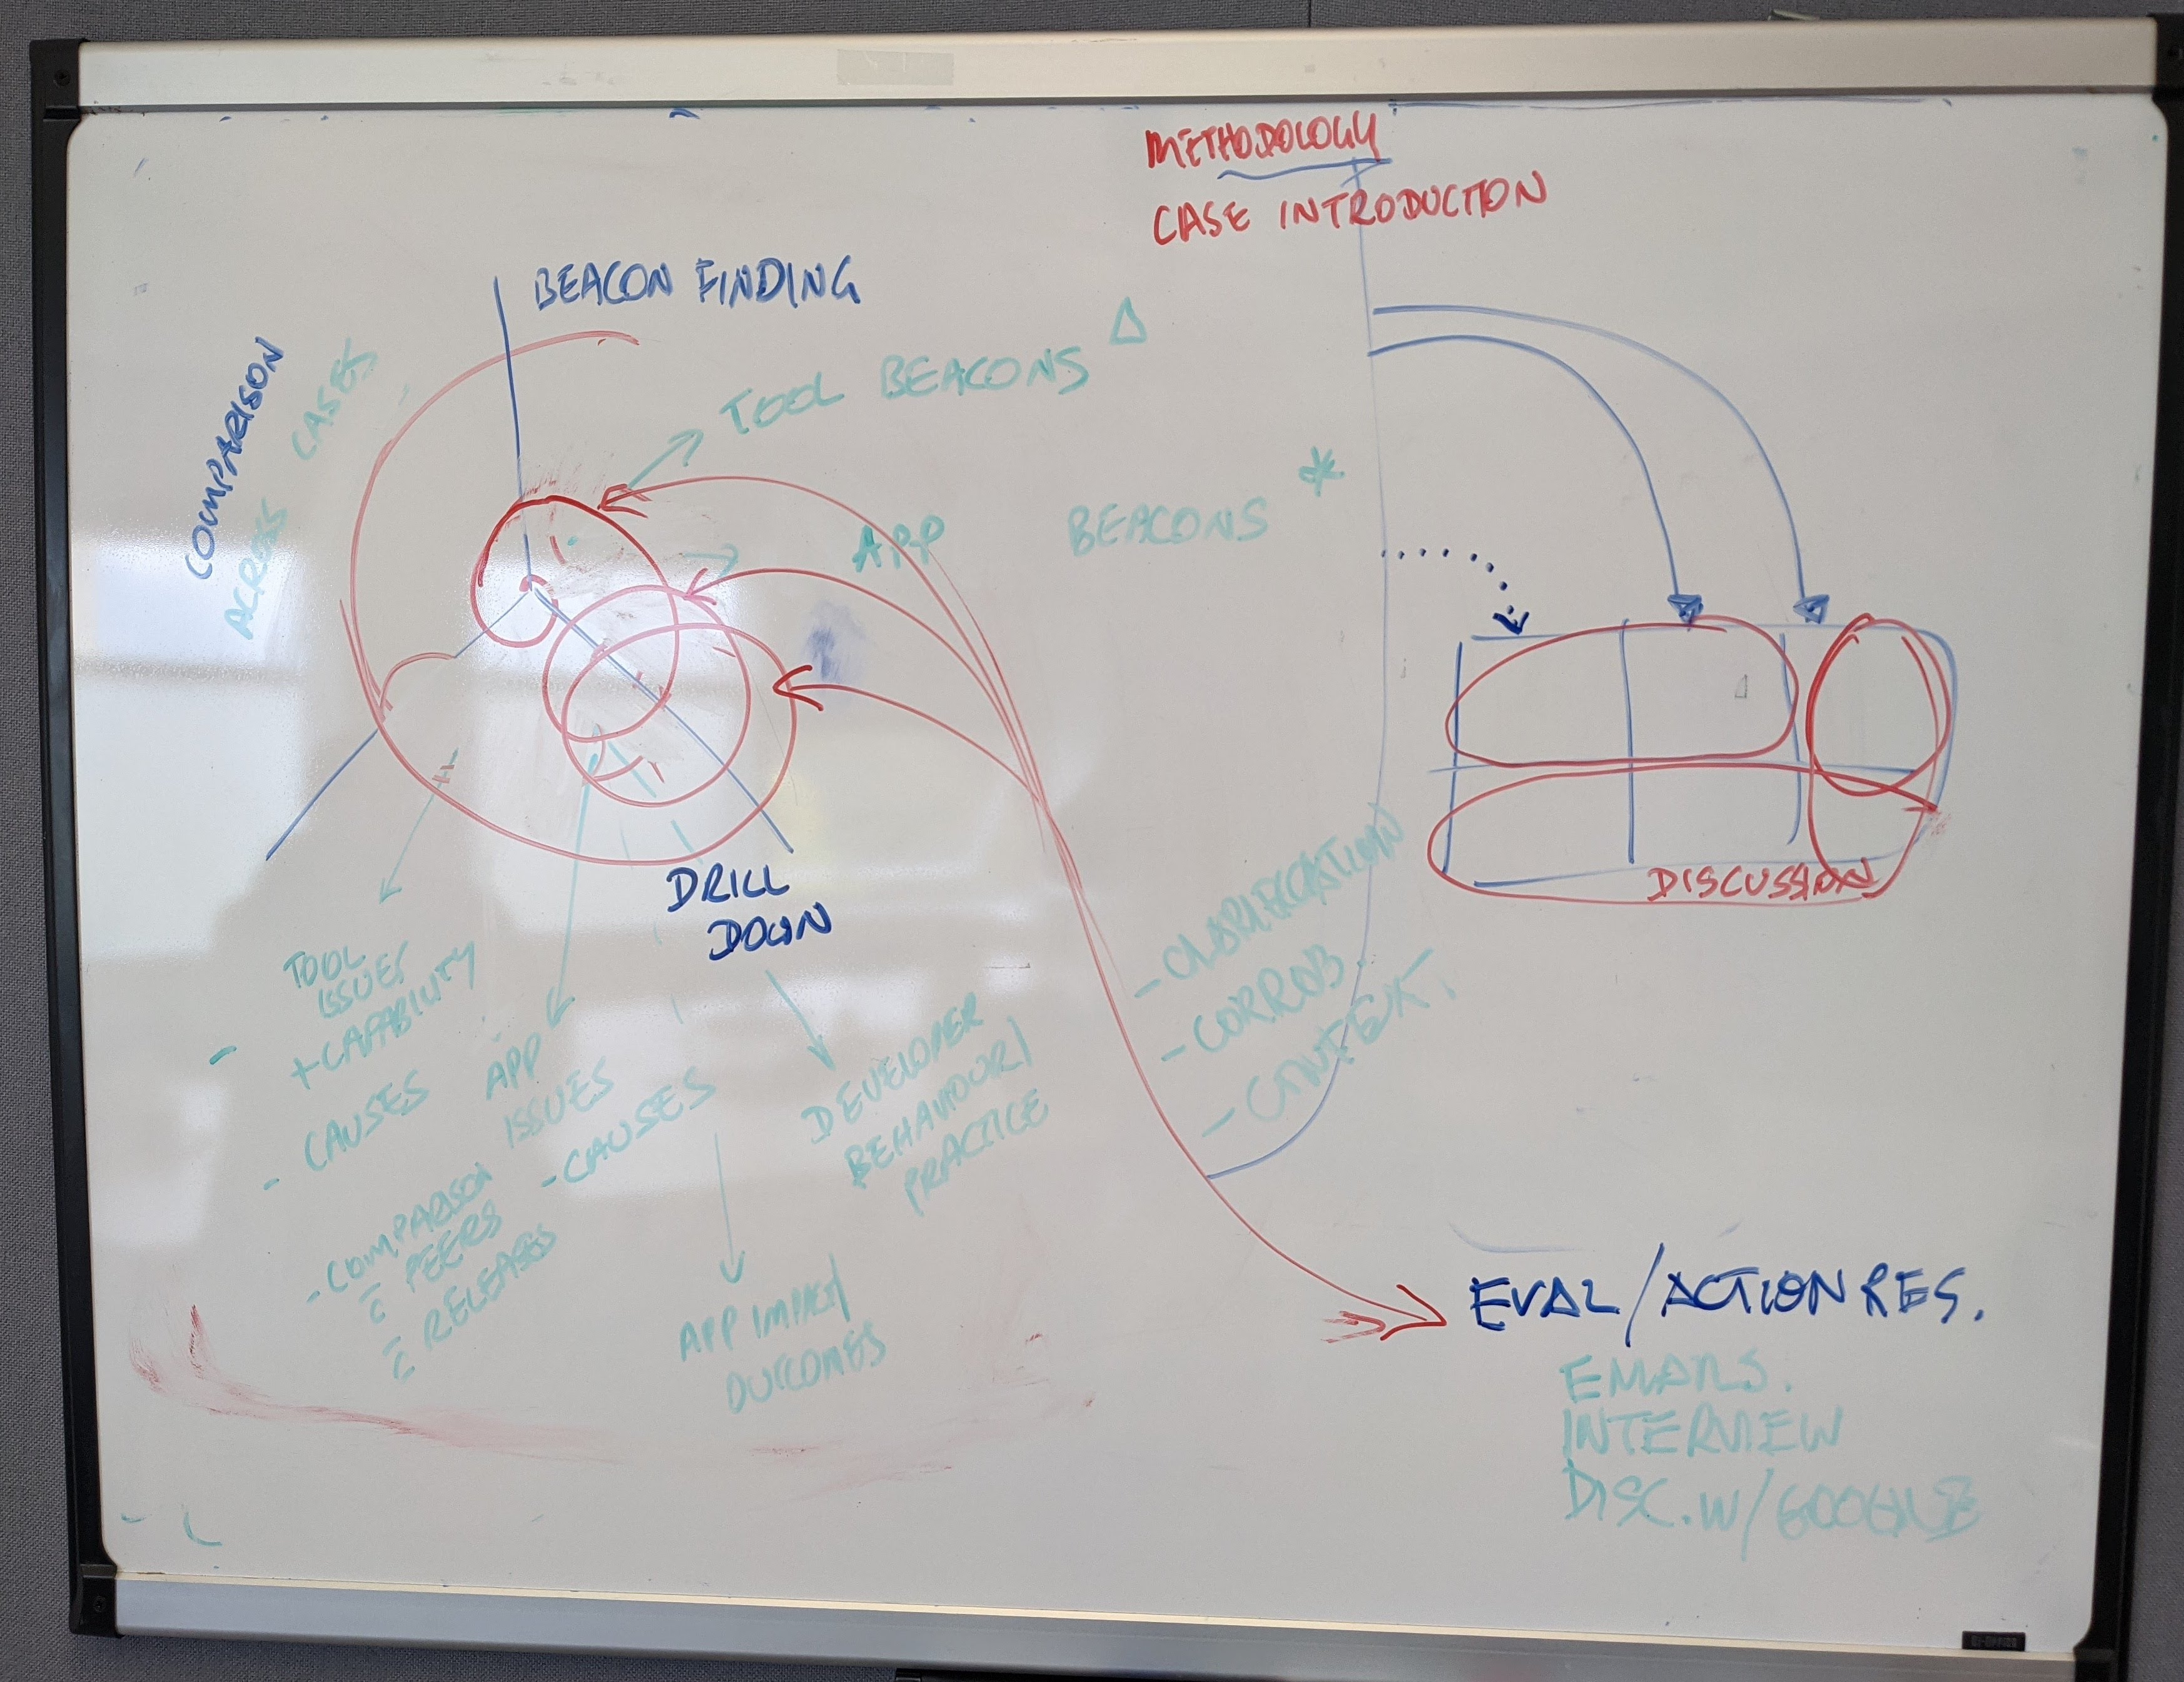
\includegraphics[width=14cm]{images/my/illustrated-combined-methodology-v0-1.jpg}
    \caption{Illustrated combined methodology}
    \label{fig:illustrated-combined-methodology}
\end{figure}

This corresponds in principle to the structure and premises of grounded theory where patterns are induced, data iterated to see if categories are appropriate, identifying patterns with comparisons with other data sets for checks and balances. 

TODO discuss saturation briefly. 

Not only could this be connected to context, it could be applied in practice to see the effects of the results.

Need to map methods to perspective. 



\section{Introducing the empirical studies}~\label{section-introducing-the-case-studies}
The case studies range in the richness of their contributions to the research, Table~\ref{tab:empirical-studies-research-perspective} provides the research context for each of them. 

\begin{landscape} % Rotates the table into a landscape page in the generate PDF
\begin{table}
    \centering
    \tabcolsep=0.06cm
    \tiny
    \begin{tabular}{lllll}\toprule
    Case Study                 & Role of Researcher &  Primary Research Method   & Research Opportunities             & Research Purpose \\
    \midrule
    Kiwix (Kiwix app)          & Embedded           & Field-experiment   & The proof-of-concept      & The treatment \\ 
    Kiwix (WikiMed (EN))       & Observer           &                    & Control for the above app & The control  \\
    Kiwix (Custom apps)        & Observer           &                    & Evaluate scalability      & \textit{pico} generalisation \\
    \midrule
    Catrobat (PocketCode)      & Coach              & Field-experiment   & Fabric Crashlytics        & Compare Mobile Analytics with Clean Code \\
    Catrobat (PocketPaint)     & Observer           &                    & Establish baseline        & The control  \\
     \midrule
    C1                         & Consultant         & Hybrid/Mixed & Large scale, complex, commercial & Mission-critical view \\
    \midrule
    GTAF                       & Interviewer        & Semi-structured interview & Add'l perspective & Exploring the long tail \\
    LocalHalo                  & Interviewer        & Semi-structured interview & Add'l technologies & Hybrid Programming and tools \\
    Moodspace                  & Interviewer        & Semi-structured interview & Small startup &Bootstrap view \\
    Moonpig                    & Interviewer        & Semi-structured interview & Leading edge view & Mature, innovative, vanguard dev. practices \\
    \midrule
    Analytics tool providers   & Various            & & `Behind the curtain' & Learn about the providers' perspectives \\
    \bottomrule
    \end{tabular}
    \caption{Empirical Studies: the research perspective}
    \label{tab:empirical-studies-research-perspective}
\end{table}
\end{landscape}

The research includes seven app-centric case studies, they are grouped into interviews and interventions. The app-centric cases were complemented by empirical studies with several providers of mobile analytics tools. Several of these initiated either directly or indirectly from the app-centric cases. 

As Table~\ref{tab:empirical-studies-research-perspective} indicates, four project teams were interviewed to provide the developers' perspectives on their use of various mobile analytics tools. Two of these (LocalHalo and GTAF) provided real-time access to at least one of these tools. GTAF also provided access to their bug tracking system which records issues they find using mobile analytics.

Three project teams were subject to interventions. Of these, both Kiwix and Catrobat develop and work as opensource projects where access to their code, to their issue tracking, and to other aspects of their projects are public. They both also provided access to their mobile analytics tools. The last of these case studies is based on a mission-critical commercial product where a similar approach to applying mobile analytics was applied for the Android app element of the product.

The tool-centric empirical studies include: Google (initiated through findings on the Kiwix and Catrobat case studies), Iteratively (who sought out the researcher, learned about the research, and were happy to share their tools and some of their commercial research), and several mobile analytics providers who provide at least some of their material as opensource. 


\section{Case study procedure}~\label{section-case-study-procedure}
% I'm not yet decided on whether to call this a: 1) methodology, model, procedure, or a technique - aspects of each of these apply to the following. See \url{https://wikidiff.com/technique/procedure} to compare two of these words, it also facilitates similar comparisons of the rest.

The case studies have several phases, this section explains each of the main phases.

The procedure needs to address the phases of each case study that involves projects and their respective organisation; namely: exploration and selection, engagement, the active case study (including data collection, contemporary analysis, and any contributions to the project), \emph{post-hoc} analysis, wrap-up, and publication. These phases may overlap somewhat, they are in approximate time order from first to last. They are covered in order in the following subsections, after the \emph{modus operandi}.

\newthought{\textit{modus operandi}}
During the active case studies, available systems are checked on multiple occasions. Pertinent examples were saved (rather than saving the contents of every check). Preserving the contents of every check may be counter-productive and risk overwhelming the researcher while providing little or no value in terms of the research results. 

In contrast, verification with the project team of actions, agreements, and analysis \emph{etc.} is appropriate and useful.

There is a tension between a) collecting potential evidence and b) the development/project practices. These may be exacerbated by the restrictions and constraints that frame each case study. Therefore, where practical a good starting point is to use existing sources of evidence (such as source code repositories, issue tracking databases, and so on), as discussed later there may be various reasons why ongoing and frequent harvesting of outputs from mobile analytics services may be challenging.eam

\subsection{Exploration and selection}
The projects and their respective organisation need to develop mobile apps and be willing to have mobile analytics for their apps. For the case studies in this research every project included at least one actively used Android app in Google Play\footnote{By having an active app in Google Play they will also have access to the Google Play Console with its dashboard, Android Vitals, release tools, and other related reports. Therefore they will \emph{de-facto} have at least one source of analytics, collected by the Google Android platform.}, however the methodology may work with minor variations for other app stores and mobile platforms.

In this research I was already working as part of a development team: for the Kiwix project. The source of the other cases was through personal recommendation, two were via academia (Catrobat and Greentech Apps) and the rest via software developers in industry.

\subsection{Engagement}
The engagement phase includes discussions to determine whether the project team (and their organisation) and the researcher(s) would be willing to participate in a viable and productive case study. It is also a suitable time to agree on the role of the researcher, and on depth, scope, range, and duration of the case study. Similarly concerns and constraints need to be determined and agreed that protect all the stakeholders involved while also allowing the research to be not deliberately biased by the project team/organisation. The stakeholders may extend beyond the primary participants, for instance the end users could potentially be stakeholders in what happens during the case study.

The decisions are made mutually by the parties involved, generally the project's team and their organisation set the limits and constraints - they need to be convinced of the value of engaging in the research. That said, if their are aware their projects have excessively high error rates (for instance if they are aware of these via their mobile analytics reports) they have the motivation to participate in the research in the hope of materially reducing the error rates and furthermore they may seek the research providing an intervention in order to achieve reductions in any excessively high error rates. 

There may also need to be discussion, joint understanding, and agreement on: intellectual property rights, copyright, confidentiality, non disclosure agreements, and so on~\footnote{Note: some researchers may be introduced to these together with the ethical aspects under the term LSEPI, discussed in ~\citet{brooke2018__becoming_professional_a_university_perspective}}. Researchers may be subject to their contract with their institution, employer, and so on. The project team and organisation sometimes may be concerned about any intellectual claims by the researcher's organisation. For the research covered in this thesis copyright is retained by the researcher.

As \citet[p.324]{barroca_2018_bridging_the_gap} notes, timeliness and relevance are vital to industry partners, while they also want to guard against the research being too intrusive or too demanding of their time or other resources. Therefore the research needs to offer something of sufficient value, relevance, and timeliness to the project team and their organisation. 

The ROI of empirical research was discussed and published a relatively long time ago from the perspective of scientific and industrial views~\citet[pp54-57]{prechelt_2007_optimizing_ROI_for_empirical_SE_studies}. Investment in case studies includes dealing with the researcher and their demands so if the researcher is able to use mobile analytics tools, analyse the reports, and investigate initial findings they may reduce the burden placed on the project team and their organisation.

Fortunately research into using mobile analytics to improve the quality of their mobile apps has often provided relevant and timely contributions to the projects, particularly in the more in-depth case studies. Also the projects generally already have at least one form of mobile analytics so the incremental cost is low in terms of tooling.
 
\subsection{The action research stage}
\julian{Question to my supervisors: if the researcher's role doesn't involve intervention is it still considered action research?}

The researcher's role will affect the activities undertaken in the action research stage (see page \pageref{section-evaluation-through-action-research-method} on roles available to the researcher). All the roles support communications with the project and allow for the researcher to ask questions, offer suggestions including issues and/or code contributions, and so on. 
\begin{itemize}
    \item For interviews, the researcher actively engages in the interview with the aim of initiating topics if they have not already arisen in the interview.
    \item In a coach role, the researcher helps set the direction and helps guide the developers in the effective use of mobile analytics tools. The researcher is expected to know how to use mobile analytics tool(s) pertinent to the case study. While they may contribute artefacts occasionally doing so is not a primary objective in this role.
    \item In an active participant role, the researcher is expected to coach, to lead aspects of the project and development-related work, and to contribute artefacts. They are also likely to be actively engaged in team discussions and aspects of planning work, etc. 
\end{itemize}

If the researcher has direct access to the mobile analytics and/or other materials (such as source code, issue tracking) they can perform at least some of the research directly. Otherwise the route to mobile analytics reports and any other material available is indirect, via someone who is part of the project and collaborating in the case study. All the case studies included elements of working with and through at least one member of the project team.

If the engagement also includes contributions to the project's materials similarly the researcher may be able to contribute directly if they have write access and/or the facility to fork the codebase and create pull requests.

For the in-depth case studies where the researcher is more actively involved with the project, the research is likely to have opportunities to work with a variety of team members, and they are also more likely to have direct access to mobile analytics and at least some of the resources. Notes made during and immediately after interviews help to record what was discussed, together with any agreements, actions, or outcomes pertinent to the research and/or the project. Subsequent checking and confirmation of the discussion, for instance in a summary email to the other people in the discussion, 

\citet[p.250]{falessi2010_applying_ESE_to_sw_architecture_etc} states \emph{``there is now a growing need to systematically gather empirical evidence about the advantages or otherwise of tools and methods rather than just rely on promotional anecdotes or rhetoric."}. That was published in 2010, similarly in current times over a decade later, there is a similar growing need to gather evidence about the use of mobile analytics.

In terms of the methodology, during the active case study it is vital to collect and perform ongoing analysis of mobile analytics and whatever other materials are available. Many of these are ephemeral in nature. for instance graphs may change by the minute. There is seldom a manual for the mobile analytics outputs (\textit{e.g.} the reports), furthermore many of the reports are dependent on the underlying data and/or on changes in the underlying service, therefore the researcher often needs to iteratively learn the mobile analytics reporting in an exploratory manner. 

Third-party mobile analytics (including those provided by Google) have terms of use. These terms of use have various names, such as a policy, \textit{e.g.} for Google Play ~\citet{google_play_developer_policy_center}. These may place limitations on data collection and use of the relevant service. For the research covered in this thesis a conservative approach was used in terms of data collection to reduce the risk of consequential issues for the researcher, the project, and the stakeholders for the app. This topic and the implications are expanded on in the \secref{chapter-discussion} chapter.

The choice of tools, including the humble web browser used by the researcher, affects aspects of the ease of collection of on line reports. As an example, the screenshot capability of the Mozilla Firefox browser~\footnote{Described in \url{https://screenshots.firefox.com/}} is far richer than that provided by Google Chrome at the time of writing. Many of the reports in mobile analytics tools require extensive vertical scrolling, Firefox can capture the entire contents easily, Chrome does not. 

Similarly some content is only generated on screen on demand, in response to user actions, for example through scrolling vertically and/or paging through reports. Others are contextual and may only appear when the relevant conditions occur~\footnote{For example, the release management reports in Google Play Console appear for the first 7 days of a new release.}. Therefore, to capture the content the researcher (or their human/automated proxy) needs to perform these actions to obtain these contents and pertinent materials saved/safeguarded to facilitate longer term analysis and provide/record evidence. Note: it is not always practical or useful to record ``everything"; how much is suitable is a topic for future research. Where practical aim to collect the underlying text in addition to visual content; the text can then be processed relatively easily and without needing to be re-keyed.



%%%%% Revised ad-hoc notes during a recent call with Arosha
% Some features are contextual...
% Aim to clearly separate the active analysis vs. the post-hoc stuff for reflective analysis especially across the case studies. Arosha expects most of the research to be based on the post-hoc aspects.

From a research perspective some analysis and verification is likely to occur during the active case study period, and some happens afterwards - based on \emph{post-hoc} analysis. \textbf{MUST-DO Expand on}: Continuous, ongoing, low latency, iterative analysis, verification, course correction, efficacious communications. 

\subsection{\emph{Post-hoc} analysis}
By this stage, the active engagement with the project has tapered-off, although in some cases additional updates may be available. For instance, if there is ongoing access to mobile analytics as some projects have provided in this research and/or updates from the project team. Nonetheless, for the most part the evidence has been harvested and any active interventions have generally ceased. The time has come to perform \emph{post-hoc} analysis and verify the findings and analysis with the project team wherever practical to do so. 

\textbf{Post-hoc analysis is more research oriented, analysis the active case study is often more project oriented.} 

The nature of the active case studies where there is a need to deal effectively with ephemeral events, data, actions, \textit{etc.} on an opportunistic, often sporadic, basis biases towards tactical findings and outcomes. From a research perspective the active case study may appear messy, chaotic, and yet incomplete. 
The \textit{post-hoc} stage provides the opportunity for complementary more reflective, objective, and strategic research. It can help reduce inadvertent bias in the more immediate tactical work by seeking contraindications, alternatives, and/or mistakes and flaws.

\newthought{Establishing patterns of case studies}~\footnote{\julian{c.f. blood group types O positive, O negative, and their sometimes uni-directional ability to be substituted, etc.}}

This stage may identify patterns within and across one or more case studies. Doing so may help to generalise the research, it may also indicate gaps in the research to date and therefore opportunities to prioritise research aimed at addressing the gaps.
% X-ref to the six perspectives and the findings. What are the data sources that helped me understand the 3 status quo's and the 3 areas or improvement.
In Figure~\ref{fig:six-perspectives} six perspectives are illustrated; these perspectives may help to categorise and group various findings in the \textit{post-hoc} analysis. 

The conclusions, together with their supporting findings and their respective sources, are well worth verifying with the project team wherever practical to do so. Doing so may help protect the integrity of the work and results; it may also provide additional value for the project and the project team. 

\begin{comment}


The \emph{post-hoc} analysis is of material that has been collected, the raw evidence for the research findings. It includes any records and results, identifying patterns in and across case studies, and so on. 

\begin{itemize}
    \itemsep0em
    \item Collating similar failures: 
    \item Bug identification and localisation: Establishing potentially pertinent patterns in the reports, and characterising when a failure \emph{does and does not} occur are part of this work. Obtaining an identifying definitive boundaries may be impractical, the work is often iterative and exploratory in nature and lossy. 
    \item Ordering and ranking clusters of failures:
    \item Bug investigation:
    \item The triage process: 
    \item Comparing information sources:
    \item ...
\end{itemize}

\end{comment}


\subsection{Wrap-up}
The research will need to be wrapped up once the bulk of the research has been completed. (A possible exception is when a case study is ongoing and has no end-date.). The wrap-up can include various actions such as safeguarding and archiving evidence, unsubscribing from services provided for a given case study, reviewing findings, analysis, and conclusions with the development team (and with their organisations), preparing what is appropriate to publish in terms of evidence, and so on.

Consider redacting personal details from communications with the stakeholders; for instance, in order to provide emails as supporting evidence for quotes and/or claims made in the research. 

This stage may also provide an opportune period for retrospectives of the case study \textit{and} for the research methods and outcomes, while the case study is still topical. The outputs of the retrospective in some cases may be valuable to fellow researchers, for instance \emph{caveats} for those who follow. 

\subsection{Publication}
Given the practical and empirical nature of the research publishing for industry \emph{and} for academia can help to increase the value of the research. These audiences may have almost orthogonal needs and expectations, for instance industry is particularly interested in highly actionable findings they can apply and obtain productive improvements almost immediately, whereas publication for academia seeks rigour and prefers peer-reviewed acceptance of the material being published.

Sometimes the development teams have the time and interest to read drafts of publications pertaining to their projects. When they do they can provide additional verification of the contents and validations of the results and conclusions.

\hrulefill

\section{Threats to validity}~\label{methodology-threats-to-validity-section}
This section concentrates on threats to validity in terms of the methodology and the use of case studies. It complements the later threats to validity section in the Discussion chapter (see page \pageref{discussion-threats-to-validity-section}.

\textbf{Methodological validity}: The research combines eleven methods grouped into four categories (see Table~\ref{tab:mapping-analysis-to-six-perspectives} on page \pageref{tab:mapping-analysis-to-six-perspectives}) there may be other, additional methods available that would provide at least as relevant results. The research uses combinations of methods to provide triangulation and to compare what people say they do with what they actually do. Flick discusses triangulation in qualitative research and sums up \emph{``three modes of application for triangulation: as a validation strategy, as an approach to the generalization of discoveries, and as a route to additional knowledge."}~\citep[p.183]{flick2004_triangulation_in_qualitative_research}. In this research triangulation is used as a route to additional knowledge and as an approach to the generalisation of discoveries.

For example, as ~\citealt[pp.132-133]{Ko2015_a_practical_guide_to_controlled_experiments_of_sw_eng_tools_with_human_participants} discusses, determining usefulness of a software tool may be tricky and there is a significant risk of developers providing the answers they believe the researcher seeks. To help mitigate against the risk of similar distortion in the findings this research focuses on the actual use as seen and as described by developers (and inferred from other development artefacts).


\textbf{Ecologically validity}: the cases are ecologically valid, being real-world projects with real-world engineering desires to apply mobile analytics, \emph{i.e., ``illustrating a tool’s benefits (or lack thereof) on a real software engineering activity taken from practice"}~\citep[p.126]{Ko2015_a_practical_guide_to_controlled_experiments_of_sw_eng_tools_with_human_participants}.

TODO discuss `Views on Internal and External Validity in Empirical Software Engineering'~\citep{sigmund2015_views_on_internal_and_external_validity_in_ESE}.
